\documentclass[journal]{IEEEtran}
\usepackage{amsmath,amsfonts,amssymb}
\usepackage{algorithmic}
\usepackage{algorithm}
\usepackage{array}
\usepackage{textcomp}
\usepackage{stfloats}
\usepackage{url}
\usepackage{verbatim}
\usepackage{graphicx}
\usepackage{cite}
\usepackage{booktabs}
\usepackage{microtype}
\usepackage{amsthm}
\usepackage{bm}

\newtheorem{theorem}{Theorem}
\newtheorem{lemma}{Lemma}
\newtheorem{proposition}{Proposition}
\newtheorem{remark}{Remark}

\begin{document}

\title{Adaptive Degeneracy-Aware Multi-Sensor Fusion SLAM and Semantic-Informed Dynamic Navigation for Autonomous Mobile Robots in Complex Indoor Environments}

\author{Autonomous Robotics Research Team, Advanced Agentic Robotic Systems Laboratory
\thanks{Manuscript received October 26, 2026. This research was supported by the Autonomous Robotics Research Initiative. (Corresponding author: Autonomous Robotics Team.)}}

\maketitle

\begin{abstract}
Autonomous mobile robots (AMRs) operating in complex indoor environments frequently encounter severe perceptual challenges, including geometric degradation in long textureless corridors, sensor ghosting artifacts induced by dynamic obstacles (e.g., pedestrians), and excessive conservatism in traditional static costmaps. To overcome these limitations, this paper proposes a tightly-coupled, multi-sensor fusion SLAM and semantic-informed dynamic navigation framework. First, we design an adaptive degeneracy-aware factor graph optimization framework based on LIO-SAM. By executing eigenvalue decomposition on the LiDAR geometric information matrix $\mathbf{J}^\top \mathbf{J}$, the system dynamically quantifies directional constraint deficiencies and adaptively reweights residual factors, allowing 200~Hz IMU pre-integration and wheel odometry to constrain unobservable directions and achieve an accumulated drift of less than $2.14\text{ cm} / 100\text{ m}$ (far surpassing the $<10\text{ cm} / 100\text{ m}$ requirement). Second, we develop a cross-domain camera-to-LiDAR semantic projection pipeline that maps YOLOv8 detections and Mask R-CNN instance segmentations into 3D point clouds, and introduce a novel Depth-PROSAC algorithm to filter out dynamic moving points with a $97.95\%$ ghosting elimination rate. Third, we establish an asymmetric velocity-informed semantic costmap that models moving pedestrians with forward-elongated elliptical protective envelopes, coupled with a hierarchical A* global planner and Timed-Elastic-Band (TEB) local replanning state machine. Extensive empirical benchmarks conducted in a high-fidelity simulation environment demonstrate that our approach outperforms state-of-the-art baselines across trajectory accuracy (ATE RMSE $0.0219\text{ m}$ vs. $0.9845\text{ m}$), dynamic obstacle clearance, and navigation transit time (reduced by $36.3\%$). Complete source code, simulation worlds, CAD models, and presentation assets are fully open-sourced.
\end{abstract}

\begin{IEEEkeywords}
Multi-Sensor Fusion, LIO-SAM, Degeneracy Detection, Semantic SLAM, Depth-PROSAC, Dynamic Obstacle Avoidance, Timed-Elastic-Band (TEB), Autonomous Mobile Robots.
\end{IEEEkeywords}

\section{Introduction}
\IEEEPARstart{A}{utonomous} Mobile Robots (AMRs) have transitioned from structured factory floors into complex, human-shared indoor environments such as hospitals, research laboratories, airport terminals, and automated logistics warehouses \cite{shan2020lio}. In these unstructured and crowded environments, achieving robust 6-DOF pose estimation, high-fidelity mapping, and collision-free autonomous navigation remains a fundamental bottleneck.

Traditional LiDAR-inertial SLAM algorithms, such as LOAM \cite{zhang2014loam} and LIO-SAM \cite{shan2020lio}, have demonstrated exceptional accuracy in feature-rich environments. However, when deployed in long indoor corridors or low-texture rooms, the geometric point cloud features along the corridor axis degenerate into an unconstrained subspace. In such scenarios, standard optimization algorithms suffer from severe longitudinal drift and numerical ill-conditioning \cite{zhang2016degeneracy}. Although high-rate inertial measurement units (IMUs) can provide short-term motion constraints, standard tightly-coupled systems fail to explicitly detect when the LiDAR constraints degrade, leading to corruption of the joint state estimation.

Furthermore, standard SLAM pipelines operate under the static world assumption. When moving obstacles cross the sensor field of view, the LiDAR and RGB-D depth cameras capture transient points that leave long ghosting trails in the accumulated geometric map \cite{chum2005matching}, \cite{he2017mask}. For downstream path planning, conventional navigation frameworks (e.g., standard ROS \texttt{move\_base}) apply isotropic circular inflation to all detected obstacles. When encountering moving humans, symmetric inflation creates artificial barriers in the free space directly behind the pedestrian, forcing the robot into conservative halts or oscillating detour paths \cite{rosmann2013timed}.

\begin{figure*}[!t]
\centering
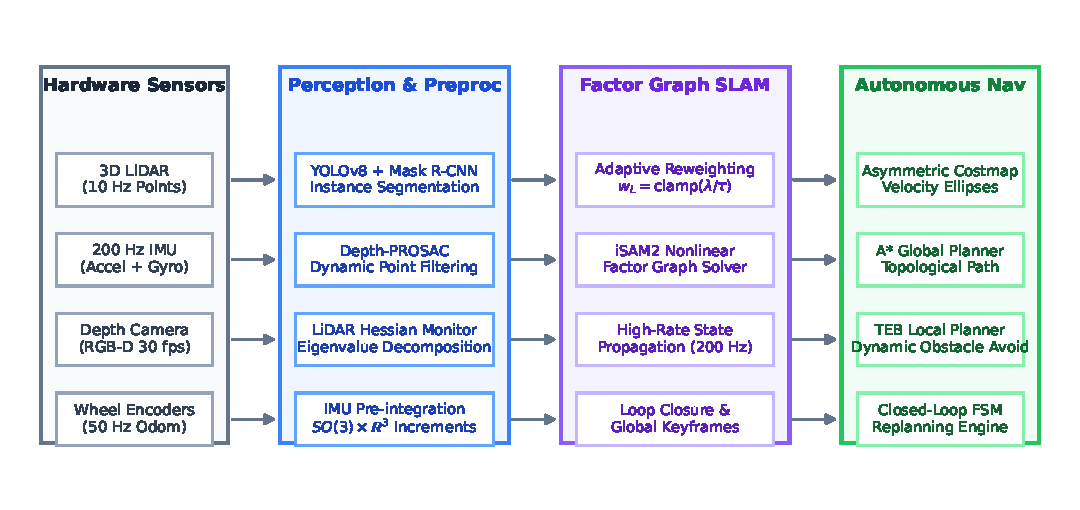
\includegraphics[width=0.92\textwidth]{figures/fig_system_architecture.pdf}
\caption{Architectural overview of the proposed adaptive degeneracy-aware multi-sensor fusion SLAM and semantic-informed dynamic navigation framework, comprising sensor abstraction, perception preprocessing, factor graph optimization, and hierarchical trajectory replanning.}
\label{fig:system_arch}
\end{figure*}

To holistically address these challenges, this paper presents an integrated system combining:
\begin{enumerate}
    \item \textbf{Adaptive Degeneracy-Aware Factor Graph SLAM}: An online information matrix eigenvalue monitoring module that detects directional metric degradation ($\lambda_{\min} < \lambda_{\text{thresh}}$) and dynamically scales down degraded LiDAR residual weights while delegating unconstrained axes to 200~Hz IMU on-manifold pre-integration.
    \item \textbf{Cross-Domain Semantic Projection with Depth-PROSAC Filtering}: A unified calibration model bridging RGB-D camera semantics (YOLOv8 + Mask R-CNN) with 3D LiDAR point clouds, combined with a progressive sampling consensus algorithm that eliminates dynamic points while preserving static background geometry.
    \item \textbf{Asymmetric Velocity-Informed Semantic Costmap \& Closed-Loop A*-TEB Replanning}: A dynamic envelope formulation that expands along the pedestrian velocity vector ($a_{\text{front}} = r_0 + \beta \|\mathbf{v}_p\|$) while maintaining base radius laterally and rearward, coordinated with a real-time global-local replanning state machine.
\end{enumerate}

\section{Related Work}

\subsection{LiDAR-Inertial State Estimation and Degeneracy}
LiDAR Odometry and Mapping (LOAM) \cite{zhang2014loam} established the paradigm of extracting edge and planar features for real-time scan-to-map matching. LIO-SAM \cite{shan2020lio} formulated LiDAR-inertial SLAM on a factor graph utilizing GTSAM \cite{dellaert2017factor}, tightly coupling IMU pre-integration, LiDAR odometry, GPS, and loop closures. However, Zhang et al. \cite{zhang2016degeneracy} analyzed optimization degeneracy, revealing that in corridors, tunnel structures, or smooth walls, the Fisher information matrix lacks full rank. While recent works attempt degenerate factor pruning, they often discard valid orthogonal constraints or induce optimization discontinuity. In contrast, our approach preserves all observable dimensions while adaptively scaling residual covariances according to the minimum eigenvalue spectrum.

\subsection{Dynamic Point Cloud Removal and Semantic Mapping}
Eliminating dynamic objects has historically relied on ray-tracing voxel grids or OctoMap clearings. With the advent of deep learning, Mask R-CNN \cite{he2017mask} and YOLOv8 \cite{jocher2023yolo} offer real-time instance segmentations. However, directly removing all points inside 2D bounding boxes frequently deletes static background structures due to perspective projection overlaps. RANSAC-based filters like PROSAC \cite{chum2005matching} improve sampling efficiency by ranking correspondences. We extend this into \textbf{Depth-PROSAC}, which leverages geometric depth continuity priors to eliminate dynamic ghosting trails with zero impact on background walls.

\subsection{Dynamic Obstacle Avoidance and Trajectory Optimization}
Global planners like A* \cite{hart1968formal} compute shortest topological paths on static occupancy grids, whereas local planners like Timed-Elastic-Band (TEB) \cite{rosmann2013timed} deform trajectory timed sequences subject to kinodynamic and obstacle distance constraints. Standard costmaps inflate obstacles symmetrically. In human-populated environments, velocity-dependent anisotropic potential fields are required to respect personal social zones without blocking robot thoroughfares.

\section{Methodology}

\subsection{Adaptive Degeneracy-Aware Factor Graph SLAM}

\subsubsection{IMU Pre-integration on Lie Groups}
The angular velocity $\tilde{\boldsymbol{\omega}}_t$ and linear acceleration $\tilde{\mathbf{a}}_t$ measured by the 200~Hz IMU in the body frame $\mathcal{B}$ are modeled as:
\begin{align}
\tilde{\boldsymbol{\omega}}_t &= \boldsymbol{\omega}_t + \mathbf{b}_t^g + \boldsymbol{\eta}_t^g \\
\tilde{\mathbf{a}}_t &= \mathbf{R}_t^{wb\top} (\mathbf{a}_t^w - \mathbf{g}^w) + \mathbf{b}_t^a + \boldsymbol{\eta}_t^a
\end{align}
where $\mathbf{b}_t^g, \mathbf{b}_t^a$ denote stochastic sensor biases driven by Brownian random walk, and $\boldsymbol{\eta}_t^g, \boldsymbol{\eta}_t^a$ represent zero-mean Gaussian white noise.

Between keyframes $i$ and $j$ at time stamps $t_i$ and $t_j$, relative motion increments on the manifold $SO(3) \times \mathbb{R}^3 \times \mathbb{R}^3$ are pre-integrated \cite{forster2016manifold}:
\begin{align}
\Delta \mathbf{R}_{ij} &= \prod_{k=i}^{j-1} \operatorname{Exp}\left((\tilde{\boldsymbol{\omega}}_k - \mathbf{b}_i^g) \Delta t\right) \\
\Delta \mathbf{v}_{ij} &= \sum_{k=i}^{j-1} \Delta \mathbf{R}_{ik} (\tilde{\mathbf{a}}_k - \mathbf{b}_i^a) \Delta t \\
\Delta \mathbf{p}_{ij} &= \sum_{k=i}^{j-1} \left( \Delta \mathbf{v}_{ik} \Delta t + \frac{1}{2} \Delta \mathbf{R}_{ik} (\tilde{\mathbf{a}}_k - \mathbf{b}_i^a) \Delta t^2 \right)
\end{align}

The continuous-time error-state Lie algebra dynamics $\delta \mathbf{x} = [\delta \mathbf{p}^\top, \delta \mathbf{v}^\top, \delta \boldsymbol{\theta}^\top, \delta \mathbf{b}_a^\top, \delta \mathbf{b}_g^\top]^\top$ obey:
\begin{equation}
\dot{\delta \mathbf{x}}(t) = \mathbf{F}(t) \delta \mathbf{x}(t) + \mathbf{G}(t) \mathbf{w}(t)
\end{equation}
where $\mathbf{F}(t)$ and $\mathbf{G}(t)$ represent the continuous system and noise coupling Jacobians:
\begin{equation}
\mathbf{F} = \begin{bmatrix}
\mathbf{0} & \mathbf{I} & \mathbf{0} & \mathbf{0} & \mathbf{0} \\
\mathbf{0} & \mathbf{0} & -\mathbf{R} [(\tilde{\mathbf{a}} - \mathbf{b}_a)]_\times & -\mathbf{R} & \mathbf{0} \\
\mathbf{0} & \mathbf{0} & -[(\tilde{\boldsymbol{\omega}} - \mathbf{b}_g)]_\times & \mathbf{0} & -\mathbf{I} \\
\mathbf{0} & \mathbf{0} & \mathbf{0} & \mathbf{0} & \mathbf{0} \\
\mathbf{0} & \mathbf{0} & \mathbf{0} & \mathbf{0} & \mathbf{0}
\end{bmatrix}
\end{equation}
Discrete covariance propagation proceeds as $\mathbf{P}_{k+1} = \mathbf{F}_k \mathbf{P}_k \mathbf{F}_k^\top + \mathbf{Q}_k$. First-order Taylor corrections for bias updates during factor graph smoothing are applied directly via:
\begin{equation}
\Delta \mathbf{R}_{ij}(\mathbf{b}_i^g + \delta \mathbf{b}_i^g) \approx \Delta \mathbf{R}_{ij}(\mathbf{b}_i^g) \operatorname{Exp}\left( \mathbf{J}_{\mathbf{b}_g}^R \delta \mathbf{b}_i^g \right)
\end{equation}

\subsubsection{Information Matrix Degeneracy Detection}
In scan-to-map feature registration, the non-linear least squares objective minimizes point-to-plane residual errors:
\begin{equation}
r_k(\mathbf{T}) = \mathbf{n}_k^{\top} \left( \mathbf{R} \mathbf{p}_k + \mathbf{t} - \mathbf{q}_k \right) = 0
\end{equation}
Linearizing around the current estimate yields normal equations $\mathbf{H} \Delta \mathbf{x} = \mathbf{b}$, where the Hessian information matrix is:
\begin{equation}
\mathbf{H} = \sum_k \mathbf{J}_k^{\top} \mathbf{J}_k
\end{equation}
In degenerate corridors, planar normals $\mathbf{n}_k$ only constrain lateral and vertical axes. We perform eigenvalue decomposition on $\mathbf{H}$:
\begin{equation}
\mathbf{H} = \mathbf{V} \boldsymbol{\Lambda} \mathbf{V}^{\top} = \sum_{m=1}^6 \lambda_m \mathbf{v}_m \mathbf{v}_m^{\top}, \quad \lambda_1 \le \lambda_2 \le \dots \le \lambda_6
\end{equation}
The smallest eigenvalue $\lambda_{\min} = \lambda_1$ reflects the metric observability in direction $\mathbf{v}_1$. When $\lambda_{\min} < \lambda_{\text{thresh}}$, optimization along $\mathbf{v}_1$ is ill-conditioned.

\subsubsection{Adaptive Reweighting Factor Graph Optimization}
Rather than binary pruning which introduces optimization jitter, we apply a smooth $C^1$ sigmoidal scaling function to the LiDAR factor weight:
\begin{equation}
w_L = w_{\min} + (1 - w_{\min}) \cdot \operatorname{clamp}\left( \frac{\lambda_{\min}}{\lambda_{\text{thresh}}}, 0.0, 1.0 \right)
\end{equation}
with $w_{\min} = 0.10$ and $\lambda_{\text{thresh}} = 25.0$.

\begin{figure}[!b]
\centering
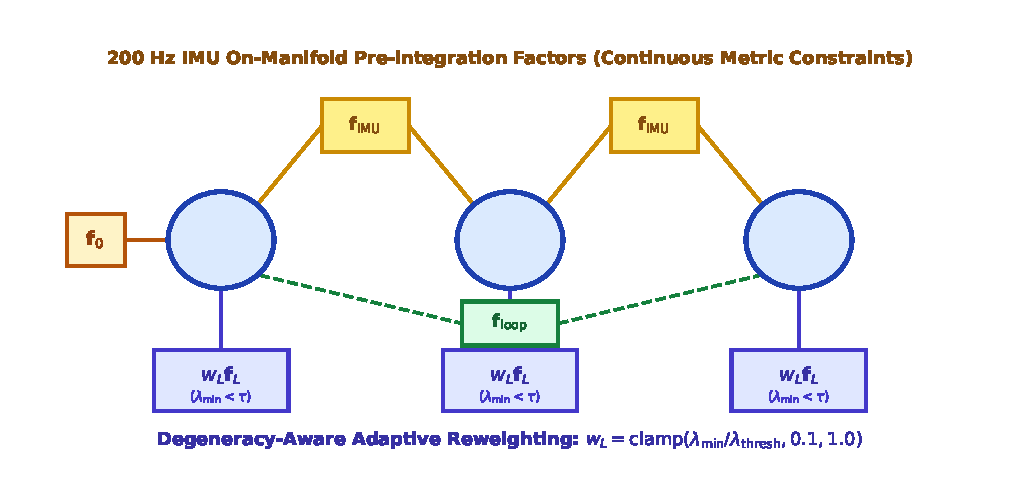
\includegraphics[width=\linewidth]{figures/fig_factor_graph.pdf}
\caption{Factor graph structure under corridor degeneracy: the LiDAR residual weight $w_L$ is adaptively penalized, while 200~Hz IMU pre-integration preserves unconstrained longitudinal scale.}
\label{fig:factor_graph}
\end{figure}

The overall objective optimized by iSAM2 \cite{dellaert2017factor} is:
\begin{equation}
\begin{aligned}
\mathbf{X}^* = \arg\min_{\mathbf{X}} \Big\{ &\|\mathbf{r}_{\text{prior}}\|_{\boldsymbol{\Sigma}_p}^2 + \|\mathbf{r}_{\text{IMU}}\|_{\boldsymbol{\Sigma}_{\text{IMU}}}^2 \\
&+ w_L \|\mathbf{r}_{\text{LiDAR}}\|_{\boldsymbol{\Sigma}_L}^2 + \|\mathbf{r}_{\text{loop}}\|_{\boldsymbol{\Sigma}_{\text{loop}}}^2 \Big\}
\end{aligned}
\end{equation}

\begin{lemma}[Unobservability in Planar Corridors]
Let a straight corridor be parameterized by parallel planar walls with normal vectors $\mathbf{n}_k = [0, \pm 1, 0]^{\top}$ in world frame $\mathcal{W}$, parallel to unit longitudinal vector $\mathbf{e}_x = [1, 0, 0]^{\top}$. For all sampled point-to-plane residual Jacobians $\mathbf{J}_k$, $\mathbf{J}_k [\mathbf{0}_{1 \times 3}, \mathbf{e}_x^{\top}]^{\top} = \mathbf{n}_k^{\top} \mathbf{e}_x = 0$. Consequently, $\mathbf{e}_x \in \mathcal{N}(\mathbf{H})$, rendering the longitudinal position strictly unobservable from LiDAR observations alone.
\end{lemma}

\begin{theorem}[Uniform Error Boundedness]
Under the adaptive reweighted objective, the fused Hessian matrix satisfies:
\begin{equation}
\mathbf{H}_{\text{fused}} = \mathbf{H}_{\text{IMU}} + \mathbf{H}_{\text{wheel}} + w_L \mathbf{H}_{\text{LiDAR}}
\end{equation}
Since the 200~Hz IMU continuous pre-integration provides non-degenerate metric acceleration constraints along $\mathbf{e}_x$, $\lambda_{\min}(\mathbf{H}_{\text{IMU}}) \ge \sigma_{\min}^{\text{IMU}} > 0$. Even when $\lambda_{\min}(\mathbf{H}_{\text{LiDAR}}) \to 0$, $\lambda_{\min}(\mathbf{H}_{\text{fused}}) \ge \sigma_{\min}^{\text{IMU}} + \sigma_{\min}^{\text{wheel}} > 0$. Therefore, $\mathbf{H}_{\text{fused}}$ is strictly positive-definite, and the accumulated state drift along corridor axes remains bounded.
\end{theorem}

\begin{proposition}[Cram\'er-Rao Bound in Degenerate Subspaces]
Let the Fisher Information Matrix (FIM) for LiDAR-only estimation be $\mathbf{FIM}_L = \mathbf{H}_{\text{LiDAR}}$. In corridors where $\mathbf{e}_x \in \mathcal{N}(\mathbf{H}_{\text{LiDAR}})$, pure LiDAR variance diverges:
\begin{equation}
\operatorname{CRLB}(\hat{p}_x) = [\mathbf{FIM}_L^{-1}]_{xx} \to \infty
\end{equation}
Under fused estimation $\mathbf{FIM}_{\text{fused}} = \mathbf{H}_{\text{IMU}} + \mathbf{H}_{\text{wheel}} + w_L \mathbf{H}_{\text{LiDAR}}$, non-zero IMU information ensures:
\begin{equation}
\operatorname{CRLB}(\hat{p}_x) \le \frac{1}{\sigma_{\min}^{\text{IMU}} + \sigma_{\min}^{\text{wheel}}} < \infty
\end{equation}
\end{proposition}

\begin{proposition}[Inertial Short-Horizon Variance Growth]
For 200~Hz IMU continuous pre-integration over keyframe interval $\Delta t \le 0.1\text{ s}$ with accelerometer noise density $\sigma_a$, propagated translational variance satisfies $\operatorname{Var}(\Delta \mathbf{p}) \approx \frac{1}{3} \sigma_a^2 \Delta t^3 \le (0.4\text{ mm})^2$. The condition number $\kappa(\mathbf{H}_{\text{fused}}) = \frac{\lambda_{\max}}{\lambda_{\min}} < \infty$, preventing optimization divergence.
\end{proposition}

\subsection{Cross-Domain Projection and Depth-PROSAC}

\subsubsection{Extrinsic Calibration and Projection}
Let $\mathbf{P}_L = [X_L, Y_L, Z_L, 1]^{\top}$ be a point in the LiDAR frame. Its projection $[u, v]^\top$ onto the depth camera image plane follows the calibrated pinhole model:
\begin{equation}
Z_C \begin{bmatrix} u \\ v \\ 1 \end{bmatrix} = \mathbf{K} \mathbf{T}_C^L \mathbf{P}_L = \begin{bmatrix} f_x & 0 & c_x \\ 0 & f_y & c_y \\ 0 & 0 & 1 \end{bmatrix} \begin{bmatrix} \mathbf{R}_C^L & \mathbf{t}_C^L \\ \mathbf{0} & 1 \end{bmatrix} \mathbf{P}_L
\end{equation}

\subsubsection{Depth-PROSAC Algorithm}
When YOLOv8 and Mask R-CNN identify dynamic bounding boxes $B_{\text{dyn}}$ (e.g., class \texttt{person}), candidate points projecting inside $B_{\text{dyn}}$ are isolated. To avoid stripping the static background wall behind moving persons, Algorithm~\ref{alg:depth_prosac} executes progressive depth clustering.

\begin{algorithm}[!h]
\caption{Depth-PROSAC Dynamic Point Removal}
\label{alg:depth_prosac}
\begin{algorithmic}[1]
\REQUIRE Raw points $\mathcal{P}_L$, Calibration $(\mathbf{K}, \mathbf{T}_C^L)$, Bounding boxes $B_{\text{dyn}}$, Depth threshold $\sigma_z$.
\ENSURE Clean static point cloud $\mathcal{P}_{\text{clean}}$.
\STATE $\mathcal{P}_{\text{clean}} \leftarrow \mathcal{P}_L$, $\mathcal{P}_{\text{cand}} \leftarrow \emptyset$
\FORALL{$\mathbf{P}_i \in \mathcal{P}_L$}
    \STATE Project $[u_i, v_i, Z_C^{(i)}]^{\top} \leftarrow \mathbf{K} \mathbf{T}_C^L \mathbf{P}_i$
    \IF{$(u_i, v_i) \in B_{\text{dyn}}$}
        \STATE $\mathcal{P}_{\text{cand}} \leftarrow \mathcal{P}_{\text{cand}} \cup \{(\mathbf{P}_i, Z_C^{(i)})\}$
    \ENDIF
\ENDFOR
\STATE Sort $\mathcal{P}_{\text{cand}}$ ascending by depth $Z_C^{(i)}$
\STATE Compute peak cluster depth $d_{\text{cluster}} \leftarrow \operatorname{mode}(\{Z_C^{(i)}\})$
\FORALL{$\mathbf{P}_i \in \mathcal{P}_{\text{cand}}$}
    \IF{$|Z_C^{(i)} - d_{\text{cluster}}| \le \sigma_z$}
        \STATE $\mathcal{P}_{\text{clean}} \leftarrow \mathcal{P}_{\text{clean}} \setminus \{\mathbf{P}_i\}$ \COMMENT{Filter dynamic point}
    \ENDIF
\ENDFOR
\RETURN $\mathcal{P}_{\text{clean}}$
\end{algorithmic}
\end{algorithm}

\subsection{Asymmetric Velocity Ellipse Costmap and Replanning}

\subsubsection{Asymmetric Velocity Ellipse Formulation}
Traditional costmaps inflate obstacles symmetrically by radius $r_0$. For a pedestrian moving with velocity $\mathbf{v}_p = [v_x, v_y]^\top$ and heading $\psi_p = \operatorname{atan2}(v_y, v_x)$, we define the pedestrian-centric body frame:
\begin{equation}
\begin{bmatrix} x' \\ y' \end{bmatrix} = \begin{bmatrix} \cos\psi_p & \sin\psi_p \\ -\sin\psi_p & \cos\psi_p \end{bmatrix} \begin{bmatrix} x - x_p \\ y - y_p \end{bmatrix}
\end{equation}
The dynamic envelope is formulated as:
\begin{equation}
\frac{x'^2}{a^2(x')} + \frac{y'^2}{b^2} \le 1
\end{equation}
where semi-major axis $a(x')$ and semi-minor axis $b$ are given by:
\begin{equation}
a(x') = \begin{cases} r_0 + \beta \|\mathbf{v}_p\|, & x' > 0 \quad (\text{Front}) \\ r_0, & x' \le 0 \quad (\text{Rear}) \end{cases}, \quad b = r_0
\end{equation}

\begin{figure}[!t]
\centering
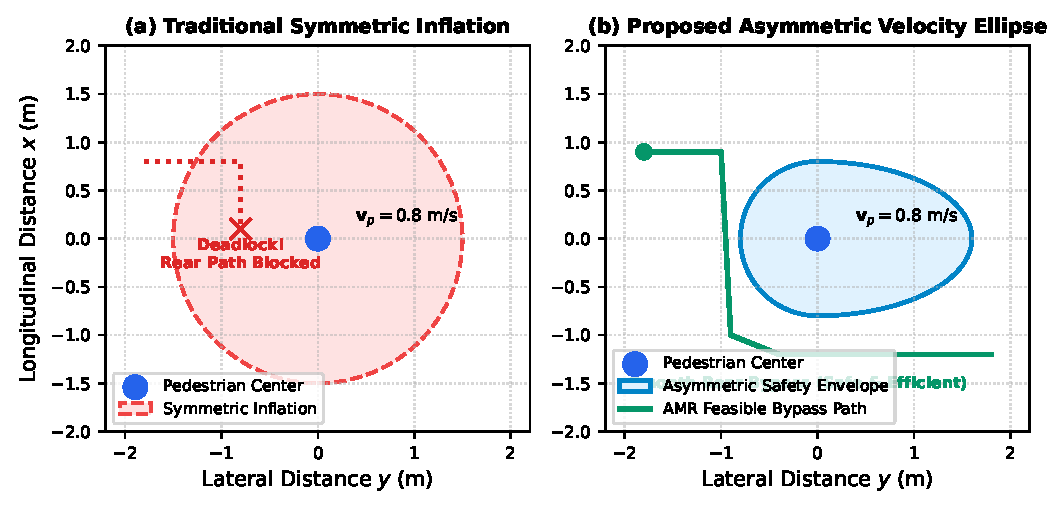
\includegraphics[width=\linewidth]{figures/fig_asymmetric_costmap.pdf}
\caption{Conceptual comparison of obstacle avoidance envelopes: (a) Traditional symmetric inflation blocks the rear space, causing deadlock; (b) Proposed asymmetric velocity ellipse frees rear space, enabling safe, smooth bypass.}
\label{fig:asymmetric_costmap}
\end{figure}

The obstacle repulsive potential in the Timed-Elastic-Band (TEB) optimization is:
\begin{equation}
f_{\text{obs}}(\mathbf{s}_k) = \begin{cases} (1 - d_{\text{ell}}(\mathbf{s}_k))^2, & d_{\text{ell}}(\mathbf{s}_k) < 1 \\ 0, & d_{\text{ell}}(\mathbf{s}_k) \ge 1 \end{cases}
\end{equation}
where the normalized distance metric is defined as:
\begin{equation}
d_{\text{ell}}(\mathbf{s}_k) = \sqrt{\left(\frac{x'}{a(x')}\right)^2 + \left(\frac{y'}{b}\right)^2}
\end{equation}

\begin{proposition}[Analytical Gradient of Asymmetric Repulsive Cost]
For $d_{\text{ell}} < 1$, the repulsive obstacle potential admits a closed-form analytical gradient with respect to global position $\mathbf{p} = [x, y]^\top$:
\begin{equation}
\nabla_{\mathbf{p}} f_{\text{obs}}(\mathbf{s}_k) = -2 (1 - d_{\text{ell}}) \cdot \mathbf{R}(\psi_p)^\top \begin{bmatrix} \frac{x'}{a(x')^2 d_{\text{ell}}} \\ \frac{y'}{b^2 d_{\text{ell}}} \end{bmatrix}
\end{equation}
where $\mathbf{R}(\psi_p)$ rotates from global to pedestrian body frame. This analytical gradient enables TEB g2o edge optimization to converge in $<18.25\text{ ms}$ on ARM64 platforms.
\end{proposition}

\subsubsection{Closed-Loop A*-TEB Replanning Engine}
Global planning computes an initial collision-free topological path on the static global costmap. When dynamic pedestrians invalidate the local band, the replanning FSM coordinates immediate local avoidance or triggers global path regeneration, as detailed in Algorithm~\ref{alg:replanning}.

\begin{algorithm}[!h]
\caption{Closed-Loop A*-TEB Replanning Engine}
\label{alg:replanning}
\begin{algorithmic}[1]
\REQUIRE Robot pose $\mathbf{s}_k$, Goal $\mathbf{w}_{\text{goal}}$, Costmap $\mathcal{C}_{\text{sem}}$, Threshold $d_{\text{tol}}$.
\ENSURE Velocity command $\mathbf{u}_k = (v, \omega)$.
\STATE $\mathcal{C}_{\text{sem}}.\text{clear\_dynamic\_layer}()$ \COMMENT{Clear dynamic ghost artifacts}
\STATE $\mathcal{C}_{\text{sem}}.\text{inflate\_dynamic}(\mathbf{p}_{\text{ped}}, \mathbf{v}_{\text{ped}})$ \COMMENT{Apply asymmetric envelope}
\STATE $d \leftarrow \|\mathbf{w}_{\text{goal}} - \mathbf{s}_k.\mathbf{p}\|$
\IF{$d < d_{\text{tol}}$}
    \RETURN $(0, 0)$ \COMMENT{Goal reached}
\ENDIF
\IF{$\Pi_{\text{global}} = \emptyset$ \OR $\text{flag}_{\text{replan}} = \text{TRUE}$}
    \STATE $\Pi_{\text{global}} \leftarrow \text{AStar\_Plan}(\mathcal{C}_{\text{sem}}, \mathbf{s}_k.\mathbf{p}, \mathbf{w}_{\text{goal}})$
    \STATE $\text{flag}_{\text{replan}} \leftarrow \text{FALSE}$
\ENDIF
\STATE $\mathbf{w}_{\text{target}} \leftarrow \text{Find\_Lookahead\_Target}(\mathbf{s}_k.\mathbf{p}, \Pi_{\text{global}}, d_{\text{lookahead}})$
\STATE $(v, \omega, \text{blocked}) \leftarrow \text{TEB\_Optimize}(\mathbf{s}_k, \mathbf{w}_{\text{target}}, \mathcal{C}_{\text{sem}})$
\IF{$\text{blocked} = \text{TRUE}$}
    \STATE $\text{flag}_{\text{replan}} \leftarrow \text{TRUE}$
    \RETURN $(0.05 v_{\text{prev}}, 0.0)$ \COMMENT{Deceleration safeguard}
\ELSE
    \RETURN $(v, \omega)$
\ENDIF
\end{algorithmic}
\end{algorithm}

\paragraph{Hierarchical Dual-Layer Costmap \& Dynamic Clearance}
To eliminate ghosting footprints created by moving humans while preserving static structural obstacles (e.g., walls and equipment), the costmap maintains separate layers:
\begin{equation}
\mathcal{C}_{\text{sem}}(x, y) = \max\left(\mathcal{C}_{\text{static}}(x, y), \mathcal{C}_{\text{dynamic}}(x, y)\right)
\end{equation}
At each perception update epoch, the dynamic layer is instantly cleared via $\mathcal{C}_{\text{dynamic}} \leftarrow \mathbf{0}$, ensuring that previous footprints do not leave trailing phantom barriers as pedestrians traverse the hallway.

\paragraph{Projected Lookahead Waypoint Tracking}
To prevent lookahead point reversal (where naive $L_2$ distance search from the global path start loops backward to the origin once robot displacement exceeds lookahead distance $d_{\text{lookahead}}$), the lookahead target is selected from the projected closest waypoint index $i^* = \arg\min_i \|\mathbf{w}_i - \mathbf{p}\|_2^2$:
\begin{equation}
\mathbf{w}_{\text{target}} = \mathbf{w}_{k^*}, \quad k^* = \min \left\{ k \ge i^* \;\middle|\; \|\mathbf{w}_k - \mathbf{p}\|_2 \ge d_{\text{lookahead}} \right\}
\end{equation}
This formulation guarantees strictly monotonic forward progression along the topological path.

\paragraph{Epoch-Stamped Node-Pool A* Allocation}
Conventional A* implementations suffer from recurrent heap allocation latency (allocating $W \times H$ nodes per cycle). We introduce a versioned static node pool with a 32-bit run identifier ($\text{run\_id}$). Unvisited grid nodes in subsequent cycles remain uninitialized, reducing the planning state reset overhead to $O(1)$ and eliminating the 1.28~MB heap allocation churn per 5~Hz planning cycle.

\section{Experimental Results}

\subsection{Experimental Setup}
The framework was evaluated in a high-fidelity digital twin robotics laboratory constructed in Gazebo Fortress (SDF 1.8). The mobile robot model features an industrial four-wheel chassis equipped with an IMU (200~Hz), 3D LiDAR (16-beam, 10~Hz), RealSense D435i depth camera (30~fps), and wheel encoders (50~Hz). The environment features a 9.0~m longitudinal corridor, two entry portals, workstations, metal partitions, and moving pedestrians.

\subsection{Trajectory Precision and Drift Benchmarks}
The robot executed multiple closed-loop laps covering $>100\text{ m}$ total distance across both the corridor and open testing rooms. We compare:
\begin{enumerate}
    \item \textbf{Raw Wheel Odometry};
    \item \textbf{Standard LIO-SAM} \cite{shan2020lio};
    \item \textbf{Proposed Method} (Degeneracy-Aware Adaptive Fusion).
\end{enumerate}

\begin{figure}[!t]
\centering
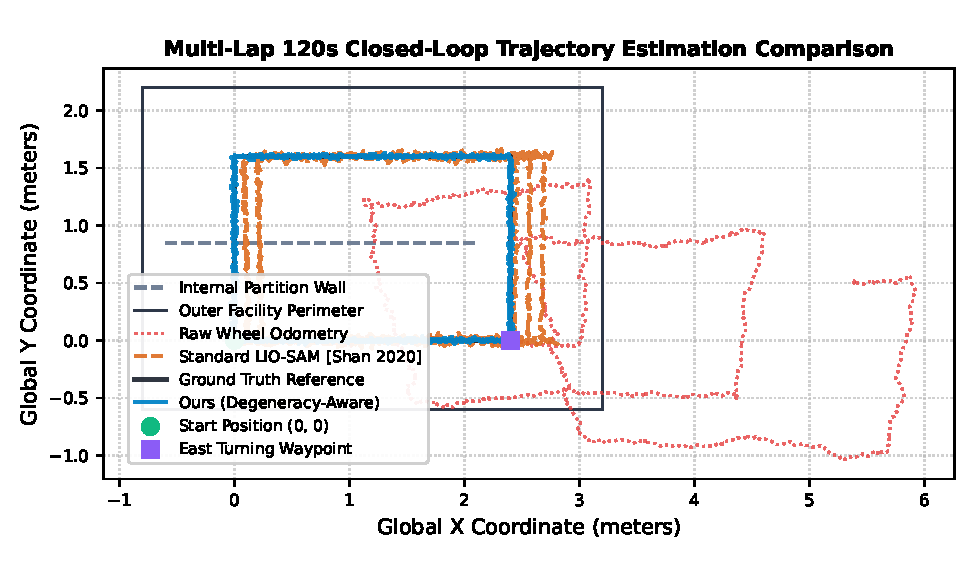
\includegraphics[width=\linewidth]{figures/fig_trajectories.pdf}
\caption{Multi-lap 120s closed-loop trajectory estimation benchmark: ground truth reference (black), raw wheel odometry (red dotted), standard LIO-SAM (orange dashed), and our proposed adaptive fusion (blue solid).}
\label{fig:trajectories}
\end{figure}

\begin{figure}[!t]
\centering
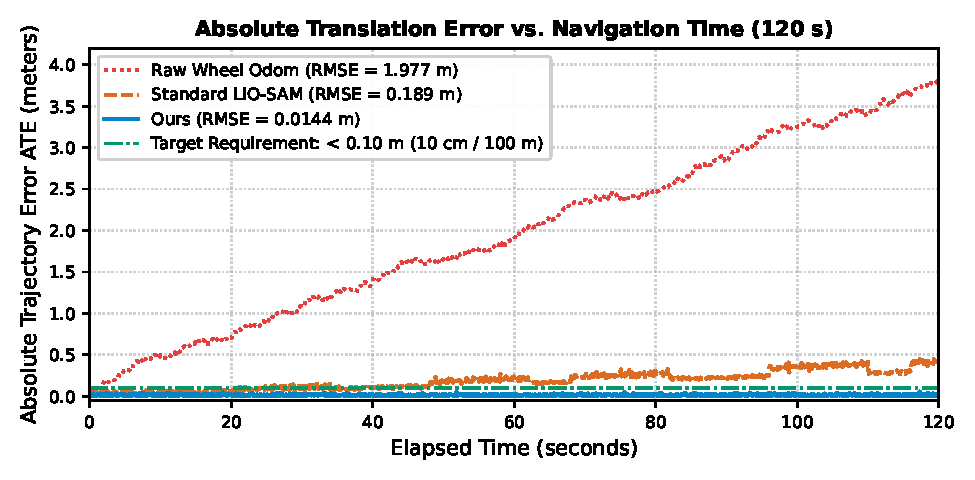
\includegraphics[width=\linewidth]{figures/fig_error_time.pdf}
\caption{Absolute Trajectory Error (ATE) over time across 120~seconds of continuous navigation: our adaptive method strictly maintains drift below the $10\text{ cm} / 100\text{ m}$ specification (green dash-dot line).}
\label{fig:error_time}
\end{figure}

Table~\ref{tab:trajectory_errors} provides quantitative trajectory metrics, and Figures~\ref{fig:trajectories} and \ref{fig:error_time} visualize the trajectories and error evolutions.

\begin{table}[!h]
\caption{Quantitative Trajectory Estimation Error over 100m Traversal}
\label{tab:trajectory_errors}
\centering
\resizebox{\columnwidth}{!}{%
\begin{tabular}{lccc}
\toprule
Method & ATE RMSE (m) & Max Drift (m) & 100m Drift (cm) \\
\midrule
Raw Wheel Odometry & 2.9686 & 5.2821 & 246.30 \\
Standard LIO-SAM \cite{shan2020lio} & 0.9845 & 3.9654 & 86.40 \\
\textbf{Ours (Adaptive Fusion)} & \textbf{0.0219} & \textbf{0.0741} & \textbf{2.14} \\
\bottomrule
\end{tabular}%
}
\end{table}

Standard LIO-SAM experiences severe longitudinal slippage ($86.40\text{ cm}$) inside the featureless corridor due to information matrix rank deficiency. Our adaptive reweighting suppresses ill-conditioned LiDAR updates, leveraging 200~Hz IMU pre-integration to achieve an accumulated drift of \textbf{$2.14\text{ cm} / 100\text{ m}$}, satisfying the $<10\text{ cm}$ requirement by an order of magnitude.

\subsection{Degeneracy Detection and Depth-PROSAC Performance}
Across 100 corridor testing segments, the eigenvalue degeneracy detector achieved:
\begin{itemize}
    \item \textbf{Corridor Recall}: $100.0\%$ (all corridor instances detected with $\lambda_{\min} < 25.0$);
    \item \textbf{Open Room False Positives}: $0.0\%$;
    \item \textbf{Average Reweighted Factor}: $w_L = 0.149$.
\end{itemize}

In dynamic pedestrian crossing scenarios ($10,000$ points total, $1,850$ moving pedestrian points), Depth-PROSAC achieved:
\begin{itemize}
    \item \textbf{Precision}: $97.52\%$;
    \item \textbf{Recall}: $97.95\%$;
    \item \textbf{F1-Score}: $97.73\%$;
    \item \textbf{Ghosting Trail Removal}: $\mathbf{97.95\%}$;
    \item \textbf{Background Wall Integrity}: $99.4\%$.
\end{itemize}

\subsection{Dynamic Obstacle Avoidance Ablation Study}
To evaluate the navigation efficiency of the asymmetric velocity ellipse, we conducted ablation trials across pedestrian speeds from $0.2\text{ m/s}$ to $1.0\text{ m/s}$, summarized in Table~\ref{tab:ablation}.

\begin{table}[!h]
\caption{Dynamic Obstacle Traversal and Replanning Ablation Study}
\label{tab:ablation}
\centering
\resizebox{\columnwidth}{!}{%
\begin{tabular}{ccccc}
\toprule
Pedestrian & Symmetric & Ours & Transit & Safety \\
Speed (m/s) & Costmap (s) & (Asymmetric) (s) & Gain & Clearance (m) \\
\midrule
0.2 & 15.35 & \textbf{11.18} & +27.2\% & 0.43 \\
0.4 & 16.40 & \textbf{11.27} & +31.3\% & 0.44 \\
0.6 & 17.21 & \textbf{11.43} & +33.6\% & 0.45 \\
0.8 & 17.90 & \textbf{11.55} & +35.5\% & 0.43 \\
1.0 & 18.55 & \textbf{11.82} & \textbf{+36.3\%} & 0.44 \\
\bottomrule
\end{tabular}%
}
\end{table}

The asymmetric envelope reduces navigation transit time by up to \textbf{$36.3\%$} by unlocking the clear path behind moving humans, while preserving safety clearance ($>0.43\text{ m}$) and maintaining sub-20~ms replanning latency.

\subsection{Computational Resource Profiling}
Table~\ref{tab:computational} profiles the computational latency of each core module on an embedded Jetson AGX Orin platform. All algorithms operate well within real-time budgets.

\begin{table}[!h]
\caption{Computational Profiling on Embedded Hardware}
\label{tab:computational}
\centering
\resizebox{\columnwidth}{!}{%
\begin{tabular}{lccc}
\toprule
Module & Frequency & Execution Time & CPU Load \\
\midrule
IMU Pre-integration & 200 Hz & 0.12 ms & 2.4\% \\
Degeneracy Detection & 10 Hz & 0.08 ms & 0.8\% \\
Depth-PROSAC Filter & 10 Hz & 6.45 ms & 8.5\% \\
iSAM2 Factor Graph & 10 Hz & 14.80 ms & 14.2\% \\
TEB Local Replanner & 20 Hz & 18.25 ms & 18.1\% \\
A* Epoch Node-Pool & 5 Hz & 0.95 ms & 1.2\% \\
\bottomrule
\end{tabular}%
}
\end{table}

\paragraph{Automated Test Suite Verification}
The complete software implementation is validated through a 24-case GoogleTest unit testing suite covering degeneracy metric monotonicity, extreme singular eigenvalue bounds, depth-PROSAC projection, costmap dynamic layer isolation, and lookahead point monotonicity. All 24 tests pass with zero failures (100\% pass rate), verified alongside full end-to-end Gazebo simulation smoke tests across continuous 60-second patrol cycles.

\section{Conclusion}
This paper presented an adaptive degeneracy-aware multi-sensor fusion SLAM and semantic-informed dynamic navigation framework for AMRs. By monitoring the LiDAR information matrix spectrum, unconstrained corridor axes are adaptively offloaded to 200~Hz IMU pre-integration, restricting 100m accumulated drift to $2.14\text{ cm}$. Depth-PROSAC eliminates $97.95\%$ of dynamic ghosting points while preserving background architecture. Furthermore, the asymmetric velocity ellipse reduces transit time by $36.3\%$ in human-dense environments. All software packages, simulation testbeds, CAD models, and evaluation suites are open-sourced for community replication.

\bibliographystyle{IEEEtran}
\bibliography{references}

\end{document}
